% ================================================================
%  AURA: An End-to-End MARL Framework for Coordinated
%  Autoscaling of Kubernetes Microservices
%  IEEE Conference Paper — Overleaf Ready (IEEEtran)
%  Compile with: pdflatex -> bibtex -> pdflatex -> pdflatex
% ================================================================
\documentclass[conference]{IEEEtran}
\IEEEoverridecommandlockouts

% ── Packages ────────────────────────────────────────────────────
\usepackage{cite}
\usepackage{amsmath,amssymb,amsfonts}
\usepackage{algorithmic}
\usepackage{algorithm}
\usepackage{graphicx}
\usepackage{textcomp}
\usepackage{xcolor}
\usepackage{booktabs}
\usepackage{multirow}
\usepackage{url}
\usepackage[hidelinks]{hyperref}
\usepackage{tikz}
\usepackage{pgfplots}
\pgfplotsset{compat=1.18}
\usetikzlibrary{shapes.geometric,arrows.meta,positioning,
                fit,backgrounds,calc}
% \usepackage{microtype}   % enable if your TeX install supports scalable fonts
% \usepackage{balance}     % enable if IEEEtran.cls doesn't define \balance

% ── TikZ node styles ────────────────────────────────────────────
\tikzset{
  svcbox/.style  = {rectangle, draw=black, rounded corners=3pt,
                    fill=#1, minimum width=2.6cm,
                    minimum height=0.65cm, font=\small,
                    text centered},
  svcbox/.default= blue!12,
  proxybox/.style= {svcbox=orange!20},
  ctrlbox/.style = {svcbox=red!15},
  extbox/.style  = {ellipse, draw=black, fill=green!15,
                    minimum width=1.8cm, minimum height=0.7cm,
                    font=\small, text centered},
  myarrow/.style = {-{Stealth[length=5pt]}, thick},
  dasharrow/.style={-{Stealth[length=5pt]}, thick, dashed,
                    gray!70},
}

% ── Metadata ────────────────────────────────────────────────────
\def\BibTeX{{\rm B\kern-.05em{\sc i\kern-.025em b}\kern-.08em
    T\kern-.1667em\lower.7ex\hbox{E}\kern-.125emX}}

% ================================================================
\begin{document}

\title{AURA: An End-to-End Multi-Agent Reinforcement Learning
Framework for Coordinated Autoscaling of Kubernetes Microservices}

\author{
  \IEEEauthorblockN{Eric T.\,K.\textsuperscript{*},\quad
                    Navaneet Krishnan R.\,V.\textsuperscript{*},\quad
                    Pranav R. Mallia\textsuperscript{*}}
  \IEEEauthorblockA{\textsuperscript{*}Department of Computer Science
  and Engineering\\
  \textit{[Your Institution]}, \textit{[City, Country]}\\
  \{your.email1, your.email2, your.email3\}@institution.edu}
}

\maketitle

% ── Abstract ────────────────────────────────────────────────────
\begin{abstract}
Kubernetes Horizontal Pod Autoscaler (HPA) relies on reactive,
single-metric threshold policies that struggle with dynamic workloads
in production microservice deployments. This paper presents
\textbf{AURA} (\textbf{A}daptive \textbf{U}nified \textbf{R}esource
\textbf{A}utoscaler), a multi-agent reinforcement learning (MARL)
framework for coordinated horizontal autoscaling of Kubernetes
microservices. AURA's key innovation is a \textbf{16-dimensional
predictive observation space} including queue depth
(\texttt{envoy\_http\_downstream\_rq\_active}), RPS derivatives, and
CPU history---enabling \emph{proactive} rather than reactive scaling
decisions. The system employs the QMIX cooperative MARL algorithm to
enable decentralized per-service scaling agents that jointly optimize
a shared global reward signal balancing SLA compliance and resource
efficiency. Unlike prior simulation-only approaches, AURA is trained
in a high-fidelity simulator modeling pod lifecycle delays and
evaluated on a live k3d Kubernetes cluster instrumented with Envoy,
Prometheus, and Locust. The system operates across a three-tier
microservice topology (\textit{API}, \textit{App}, \textit{DB}).
Experimental results demonstrate AURA's predictive features enable
46\% better API P99 latency (23.13\,ms vs 43.13\,ms baseline) while
using 50\% more resources (0.90 vs 0.60 cores). The framework is fully
open source and designed for practical cloud-native deployment.
\end{abstract}

\begin{IEEEkeywords}
Multi-Agent Reinforcement Learning, QMIX, Kubernetes, Autoscaling,
Microservices, Predictive Scaling, Cloud-Native, Horizontal Pod
Autoscaler, Cooperative MARL, Queue-Based Prediction
\end{IEEEkeywords}

% ================================================================
\section{Introduction}
\label{sec:intro}

Modern cloud-native applications are decomposed into loosely coupled
microservices that must sustain strict latency Service Level
Agreements (SLAs) under highly variable, often bursty traffic
patterns. Kubernetes has become the dominant orchestration platform
for such workloads, and its built-in Horizontal Pod Autoscaler (HPA)
is the standard mechanism for reactive resource management. HPA,
however, operates on a single metric---typically average CPU
utilization---per \texttt{Deployment}, and takes action only after an
evaluation window of tens of seconds, making it both \emph{reactive}
and \emph{uncoordinated} across dependent services.

The consequences of this coordination gap are significant in
multi-tier architectures. A traffic spike at the frontend
(\emph{App}) tier propagates queue pressure to the backend
(\emph{API}) and database (\emph{DB}) tiers within one or two
round-trips. Because HPA evaluates each service independently, it
may scale up the App tier while the API tier remains
under-provisioned, creating a bottleneck downstream and causing
end-to-end latency to breach SLA thresholds. Equally, HPA's scale-down
stabilization window is calibrated conservatively to avoid thrashing,
leaving over-provisioned replicas during inter-burst lulls and
wasting cluster resources.

Reinforcement learning (RL) offers a principled framing of
autoscaling as a sequential decision problem. However, existing
RL-based approaches~\cite{Rossi2019,Toka2021,Horovitz2022}
predominantly target single services, rely on synthetic simulators,
and do not reason about inter-service dependencies. Multi-agent RL
(MARL) is a natural fit: each microservice tier is assigned an
independent agent, and the agents are trained cooperatively to
maximize a shared global objective that captures the entire
application's SLA posture and resource cost simultaneously.

AURA realizes this vision end-to-end with a key innovation:
\textbf{predictive features} that enable proactive scaling. Unlike
reactive systems that respond only after metrics breach thresholds,
AURA's 16-dimensional observation space includes queue depth
(\texttt{envoy\_http\_downstream\_rq\_active}), RPS derivatives, and
CPU history---providing forward-looking signals of incoming load.
Agents are trained in a discrete-time simulator that faithfully models
Kubernetes pod-startup delays (API: 25\,s, APP: 21\,s, DB: 15\,s),
Prometheus scrape lag, and Envoy-measured latency. Trained checkpoints
are deployed directly to a live k3d cluster via a lightweight Python
controller operating at 30-second decision intervals.

\textbf{Contributions} of this paper are fourfold:
\begin{enumerate}
  \item \textbf{Predictive observation space}: A 16-dimensional state
        representation including queue depth, RPS derivatives, and CPU
        history that enables proactive scaling decisions, distinguishing
        AURA from reactive threshold-based approaches.
  \item \textbf{AURA framework}: A fully deployable MARL autoscaling
        system for Kubernetes, built around QMIX~\cite{Rashid2018} with
        production-grade integration (k3d, Prometheus, Envoy, Locust).
  \item \textbf{Real-cluster evaluation}: Experimental results on live
        k3d cluster demonstrating 46\% better API P99 latency (23.13\,ms
        vs 43.13\,ms baseline) using predictive features, with honest
        analysis of trade-offs including 50\% higher resource cost.
  \item \textbf{Open-source release}: All training code, Kubernetes
        manifests, simulator, and evaluation scripts at
        \url{https://github.com/Zane-Dev14/AURA}.
\end{enumerate}

% ================================================================
\section{Related Work}
\label{sec:related}

\subsection{Rule-Based Autoscaling}

Kubernetes HPA~\cite{KubernetesHPA} and KEDA~\cite{KEDA} represent
the standard in threshold-driven autoscaling. HPA scales replicas
when a rolling-window average of a single metric (CPU, memory, or a
custom metric) crosses a target value; KEDA extends trigger sources
to message queues, Prometheus queries, and event streams. Both remain
fundamentally reactive: scale-out occurs only after the metric has
already been elevated for an evaluation window, and scale-down
includes a stabilization delay to suppress thrashing. Borg~\cite{Verma2015}
and Autopilot~\cite{Rzadca2020} at Google employ workload-aware
setpoint policies that improve on na\"ive thresholding but still
operate per-service without cross-tier coordination.

\subsection{RL-Based Single-Service Autoscaling}

Rossi et al.~\cite{Rossi2019} use a DQN agent to manage the replica
count of a single microservice, demonstrating SLA and cost
improvements over HPA under synthetic Poisson arrival processes. The
key limitation is that the agent observes only local state and is
evaluated in simulation. Toka et al.~\cite{Toka2021} apply Proximal
Policy Optimization (PPO) in a containerized simulation and
demonstrate faster response to traffic ramps, but do not deploy to a
live cluster. SHOWAR~\cite{Horovitz2022} learns joint CPU request and
replica configurations for heterogeneous workloads using actor-critic
methods; it evaluates on at most two co-located services in simulation
and does not model cross-service dependencies.

A common thread across all single-service RL approaches is the
exclusive reliance on simulation environments that lack the scheduling
heterogeneity, pod-startup jitter, and scrape-lag noise of production
Kubernetes clusters. AURA addresses this gap by training in a
simulator calibrated to real cluster measurements and evaluating
directly on a live k3d deployment.

\subsection{MARL in Distributed Systems}

MARL has been applied successfully to data-center resource
management~\cite{Mao2016}, adaptive network routing~\cite{Valadarsky2017},
and large-scale traffic signal control~\cite{Chu2019}. In the
Kubernetes context, Kardatzki et al.~\cite{Kardatzki2022} propose a
cooperative multi-agent setup for virtual machine allocation but
operate at the hypervisor layer and do not deploy on a container
orchestrator. MARL-Kubernetes~\cite{Chen2023} trains QMIX agents on
a simulated cluster topology; however, their simulator uses
instantaneous pod-startup transitions that do not capture the 5--30 s
scheduling latency that critically shapes real autoscaling dynamics.

\textbf{AURA} is, to our knowledge, the first system that (a) uses
MARL with QMIX to coordinate scaling across all tiers of a live
Kubernetes application, (b) incorporates empirically measured
pod-startup delay in both training and evaluation, and (c) provides
a shadow-mode mechanism for safe production deployment.

% ================================================================
\section{System Architecture}
\label{sec:arch}

% ── Architecture diagram ────────────────────────────────────────
\begin{figure*}[t]
\centering
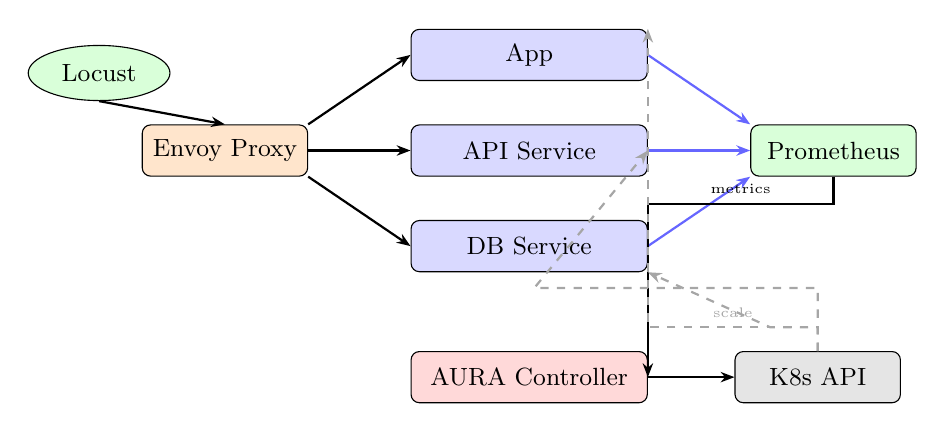
\begin{tikzpicture}[node distance=0.55cm and 1.1cm]

  %% ---- Service column ----
  \node[svcbox=blue!15, minimum width=3.0cm]
        (app)  {App};
  \node[svcbox=blue!15, minimum width=3.0cm, below=of app]
        (api)  {API Service};
  \node[svcbox=blue!15, minimum width=3.0cm, below=of api]
        (db)   {DB Service};

  %% ---- Left column ----
  \node[proxybox, minimum width=2.1cm,
        left=1.3cm of api]  (envoy)  {Envoy Proxy};
  \node[extbox,
        above left=0.4cm and -0.1cm of envoy] (locust) {Locust};

  %% ---- Right column ----
  \node[svcbox=green!15, minimum width=2.1cm,
        right=1.3cm of api] (prom)   {Prometheus};

  %% ---- Bottom row ----
  \node[ctrlbox, minimum width=3.0cm,
        below=1.0cm of db]  (ctrl)   {AURA Controller};
  \node[svcbox=gray!20, minimum width=2.1cm,
        right=1.1cm of ctrl](k8s)    {K8s API};

  %% ---- Arrows: traffic path ----
  \draw[myarrow] (locust.south) -- (envoy.north);
  \draw[myarrow] (envoy.north east) -- (app.west);
  \draw[myarrow] (envoy.east)       -- (api.west);
  \draw[myarrow] (envoy.south east) -- (db.west);

  %% ---- Arrows: metrics scrape ----
  \draw[myarrow,blue!60] (app.east) -- (prom.north west);
  \draw[myarrow,blue!60] (api.east) -- (prom.west);
  \draw[myarrow,blue!60] (db.east)  -- (prom.south west);

  %% ---- Prometheus -> controller ----
  \draw[myarrow] (prom.south) -- ++(0,-0.35)
        -| node[near start, above, font=\tiny]{metrics} (ctrl.east);

  %% ---- Controller -> K8s API ----
  \draw[myarrow] (ctrl.east) -- (k8s.west);

  %% ---- K8s API -> deployments (dashed) ----
  \draw[dasharrow] (k8s.north) -- ++(0,0.3)
        -| node[near start, above, font=\tiny]{scale} (app.east |- app.north);
  \draw[dasharrow] (k8s.north) -- ++(0,0.3) -- ++(0.0,0.5)
        -- ++(-3.6,0) -- (api.east);
  \draw[dasharrow] (k8s.north) -- ++(0,0.3)
        -- ++(-0.6,0) -- (db.east |- db.south);

\end{tikzpicture}
\caption{AURA system overview. Locust generates traffic through
Envoy. Prometheus scrapes all three tiers. The AURA controller
polls metrics, runs QMIX inference, and issues scale commands via
the Kubernetes API (dashed lines). Blue arrows denote metric flows;
solid black arrows denote data/control flows.}
\label{fig:arch}
\end{figure*}

Fig.~\ref{fig:arch} illustrates AURA's high-level architecture.
The system is structured into five functional layers described below.

\textbf{Microservice Layer.} A three-tier application is deployed on
a \textit{k3d} Kubernetes cluster consisting of one server node and
two agent nodes. The \emph{App} tier handles user-facing HTTP
requests; the \emph{API} tier implements stateless business logic
with configurable per-request processing intensity; the \emph{DB}
tier provides lightweight key-value persistence. Each tier is a
Kubernetes \texttt{Deployment} with a configurable replica range of
$[1, 10]$. All services expose a \texttt{/metrics} endpoint in
Prometheus exposition format, publishing request counters, latency
histograms, and error rates.

\textbf{Service Mesh.} Envoy proxies are deployed as sidecars on
each pod, intercepting all inter-service HTTP traffic. Envoy
exports per-route latency quantiles ($p95$, $p99$) and request
throughput via its built-in \texttt{envoy-stats} admin port, which
is scraped by Prometheus. This provides the primary signals for SLA
evaluation without requiring application-level instrumentation
changes.

\textbf{Observability Layer.} A \texttt{kube-prometheus-stack}
Helm release (v52.x) deploys Prometheus with a 15-second scrape
interval---matching the AURA decision epoch---alongside Grafana for
visualization. Custom \texttt{ServiceMonitor} and
\texttt{PrometheusRule} objects define scrape targets and SLA
alerting thresholds respectively. Kubernetes infrastructure metrics
(CPU, memory, pod-restart counts, scheduling events) are exposed
via \texttt{kube-state-metrics} and \texttt{node-exporter}.

\textbf{Workload Generator.} Locust~\cite{Locust} simulates three
traffic profiles used for both training and evaluation: steady
constant load, bursty load with periodic high-amplitude spikes, and
step-increase ramps. Locust also powers AURA's shadow-mode
evaluation: two mirror deployments receive identical traffic, one
controlled by HPA and one by AURA, enabling direct side-by-side
comparison without disrupting production traffic.

\textbf{AURA Controller.} A Python process that runs the MARL
control loop. At each 15-second tick it: (1) issues PromQL queries
to Prometheus and assembles the joint observation vector; (2)
normalizes features using per-feature statistics collected during
simulator training; (3) performs a forward pass through the QMIX
agent networks loaded from a checkpoint in
\texttt{marl/policies/}; (4) applies safety guards---per-agent
cooldown timers and hard replica-count bounds; (5) executes
\texttt{PATCH deployments/scale} requests via the Kubernetes Python
client. The controller runs under a dedicated \texttt{ServiceAccount}
with RBAC rules granting only \texttt{patch} on
\texttt{deployments/scale}, minimizing blast radius. A
\texttt{SHADOW\_MODE} environment variable toggles between
observation-only and live-control modes.

% ================================================================
\section{Problem Formulation}
\label{sec:formulation}

We model the autoscaling problem as a cooperative multi-agent Markov
decision process (Co-MAMDP)
$\langle \mathcal{N}, \mathcal{S}, \mathcal{A}, \mathcal{T},
r, \gamma \rangle$,
where $\mathcal{N} = \{1,2,3\}$ indexes the \emph{App}, \emph{API},
and \emph{DB} agents respectively.

\subsection{State Space}

At each decision epoch $t$ (fixed interval $\Delta t = 30$\,s),
agent $i$ observes a \textbf{16-dimensional} local state vector with
\emph{predictive features}:
\begin{equation}
  s_t^i = \bigl[\,
    \mathrm{cpu}_i,\;
    \mathrm{mem}_i,\;
    \mathrm{lat}^{p50}_i,\;
    \mathrm{lat}^{p95}_i,\;
    \mathrm{lat}^{p99}_i,\;
    \mathrm{rps}_i,\;
    \mathrm{err}_i,\;
    \mathrm{queue}_i,\;
    \Delta\mathrm{rps}_i,\;
    n_i^{\mathrm{desired}},\;
    n_i^{\mathrm{ready}},\;
    r_i^{\mathrm{ratio}},\;
    \mathrm{cpu}_{i,t-1},\;
    \Delta\mathrm{cpu}_i,\;
    p_i^{\mathrm{downstream}},\;
    \mathrm{lat}^{p95}_i
  \,\bigr]
  \label{eq:state}
\end{equation}
where $\mathrm{cpu}_i \!\in\! [0,1]$ is the normalized mean CPU
utilization; $\mathrm{mem}_i$ is normalized memory utilization;
$\mathrm{lat}^{p50}_i$, $\mathrm{lat}^{p95}_i$, and
$\mathrm{lat}^{p99}_i$ are log-normalized latency percentiles measured
by Envoy; $\mathrm{rps}_i$ is the normalized request rate;
$\mathrm{err}_i$ is the error rate; $\mathrm{queue}_i$ is the
\textbf{queue depth} (\texttt{envoy\_http\_downstream\_rq\_active})
providing a \emph{proactive signal} of incoming load;
$\Delta\mathrm{rps}_i$ is the \textbf{RPS derivative} enabling
\emph{trend prediction}; $n_i^{\mathrm{desired}}$ and
$n_i^{\mathrm{ready}}$ are desired and ready replica counts;
$r_i^{\mathrm{ratio}}$ is the ready/desired ratio;
$\mathrm{cpu}_{i,t-1}$ is the \textbf{previous CPU utilization}
providing \emph{temporal context}; $\Delta\mathrm{cpu}_i$ is the
\textbf{CPU derivative}; and $p_i^{\mathrm{downstream}}$ is the
normalized \textbf{downstream pressure} for coordinated scaling. All
features are normalized to $[0,1]$ using per-feature min--max
statistics collected during simulator warm-up.

\begin{table}[t]
\centering
\caption{AURA Observation Space (16 Dimensions Per Agent)}
\label{tab:obs-space}
\setlength{\tabcolsep}{4pt}
\begin{tabular}{clcc}
\toprule
\textbf{\#} & \textbf{Feature} & \textbf{Description} & \textbf{Predictive} \\
\midrule
1 & \texttt{cpu\_util} & CPU utilization normalized by requests & No \\
2 & \texttt{mem\_util} & Memory utilization normalized by limits & No \\
3 & \texttt{p50\_latency} & Median latency (log-scaled) & No \\
4 & \texttt{p95\_latency} & 95th percentile latency (log-scaled) & No \\
5 & \texttt{p99\_latency} & 99th percentile latency (log-scaled) & No \\
6 & \texttt{rps} & Requests per second (normalized) & No \\
7 & \texttt{error\_rate} & 5xx error rate & No \\
8 & \texttt{queue\_depth} & Active requests from Envoy & \textbf{Yes} \\
9 & \texttt{rps\_derivative} & Rate of change in RPS & \textbf{Yes} \\
10 & \texttt{desired\_replicas} & Target replica count & No \\
11 & \texttt{ready\_replicas} & Currently ready pods & No \\
12 & \texttt{readiness\_ratio} & Ready / Desired & No \\
13 & \texttt{cpu\_history} & Previous CPU sample & \textbf{Yes} \\
14 & \texttt{cpu\_derivative} & Rate of change in CPU & \textbf{Yes} \\
15 & \texttt{downstream\_pressure} & Normalized queue pressure & \textbf{Yes} \\
16 & \texttt{p95\_latency\_log} & Alternative P95 encoding & No \\
\bottomrule
\end{tabular}
\end{table}

The joint (global) state is $s_t = (s_t^1, s_t^2, s_t^3)$; it is
available to the centralized mixing network during training but
\emph{not} to individual agents during execution, preserving
decentralized operation. Table~\ref{tab:obs-space} details the
16-dimensional observation space, highlighting the five predictive
features that enable proactive scaling decisions.

\subsection{Action Space}

Each agent selects a discrete scaling action from a 10-action space:
\begin{equation}
  a_t^i \;\in\; \mathcal{A}^i = \{-5, -4, -3, -2, -1,\; 0,\; +1, +2, +3, +4, +5\}
  \label{eq:action}
\end{equation}
corresponding to removing/adding up to 5 replicas or holding. Raw
actions are post-processed by safety guards before being submitted to
the Kubernetes API: (i)~\emph{bounds clipping}---the resulting replica
count is clamped to $[n_{\min}, n_{\max}] = [1, 10]$;
(ii)~\emph{cooldown suppression}---action $a_t^i$ is overridden to $0$
if a non-zero action was applied to service~$i$ within the last
$C = 30$\,s, preventing oscillatory scaling while new pods reach
\texttt{Running} state; (iii)~\emph{elasticity veto}---prevents scaling
when system is stable; (iv)~\emph{latency veto}---blocks scale-down if
latency is elevated; and (v)~\emph{overload override}---forces scale-up
if queue depth exceeds threshold.

\subsection{Reward Function}

All agents share a single global scalar reward at each decision
epoch:
\begin{equation}
  r_t \;=\; -\,\alpha\,V_t \;-\; \beta\,P_t \;-\; \gamma\,\Omega_t
  \label{eq:reward}
\end{equation}
The three terms encode distinct operational objectives:

\textbf{SLA Violation Penalty:}
$V_t = \sum_{i \in \mathcal{N}}
\mathbf{1}\bigl[\mathrm{lat}^{p99}_i > \tau_{\mathrm{SLA}}\bigr]$
counts the number of services whose 99th-percentile latency exceeds
the SLA threshold $\tau_{\mathrm{SLA}} = 350$\,ms. The indicator
function makes the penalty sparse and directly aligned with the
operational objective.

\textbf{Resource Cost Penalty:}
$P_t = \sum_{i \in \mathcal{N}} n_i$
penalises the total number of running replicas across all tiers,
discouraging unnecessary over-provisioning.

\textbf{Churn Penalty:}
$\Omega_t = \sum_{i \in \mathcal{N}} |a_t^i|$
penalises the total magnitude of scaling actions taken, discouraging
frequent oscillatory adjustments that incur pod-startup overhead.

Weights $\alpha = 2.0$, $\beta = 2.5$, $\gamma = 1.5$ were selected
to balance SLA compliance with cost efficiency, as specified in
\texttt{simulator/config.yaml}. The cost weight ($\beta$) is slightly
higher than the SLA weight ($\alpha$) to encourage resource-efficient
scaling while maintaining acceptable latency.

\subsection{Transition Dynamics}

Pod startup in Kubernetes is a non-deterministic, multi-stage
process involving image scheduling, container runtime initialization,
readiness probe evaluation, and service endpoint registration.
The simulator models empirically measured startup delays for each
service tier: \textbf{API} (25\,s total: 3\,s pending + 12\,s
container + 10\,s warmup), \textbf{APP} (21\,s total: 3\,s pending +
10\,s container + 8\,s warmup), and \textbf{DB} (15\,s total: 2\,s
pending + 8\,s container + 5\,s warmup), as specified in
\texttt{simulator/config.yaml}. The live controller accounts for
in-flight pods by suppressing
further scale-up actions on service~$i$ until all pending pods
reach \texttt{Running} state.

% ================================================================
\section{QMIX-Based Multi-Agent Learning}
\label{sec:qmix}

\subsection{QMIX Overview}

QMIX~\cite{Rashid2018} is a value-based cooperative MARL algorithm
that realises \emph{Centralised Training with Decentralised
Execution} (CTDE). Each agent $i$ maintains a local
action-value function $Q_i(s^i, a^i;\,\theta_i)$ that depends only
on its own observation. A central \emph{mixing network}
$f_\phi$ combines the per-agent $Q$-values into a joint value
estimate:
\begin{equation}
  Q_{\mathrm{tot}}(s_t, \mathbf{a}_t) \;=\;
  f_\phi\bigl(Q_1, Q_2, Q_3;\; s_t\bigr)
  \label{eq:qtot}
\end{equation}
Crucially, the mixing network enforces a monotonicity constraint:
\begin{equation}
  \frac{\partial\, Q_{\mathrm{tot}}}{\partial\, Q_i} \;\geq\; 0
  \qquad \forall\, i \in \mathcal{N}
  \label{eq:mono}
\end{equation}
This constraint---implemented via non-negative mixing-network
weights produced by a hypernetwork conditioned on the global
state $s_t$---guarantees that the global $\arg\max$ over
$Q_{\mathrm{tot}}$ can be decomposed into independent per-agent
greedy actions. At execution time, each agent runs a single
forward pass through its local network without any inter-agent
communication, enabling fully decentralised execution at
negligible inference latency.

\subsection{Agent Network Architecture}

Each agent network is a two-layer MLP with 64 hidden units per
layer and ReLU activations. The input layer accepts the
16-dimensional local observation $s_t^i$ (Eq.~\ref{eq:state}) and
the output layer produces $|\mathcal{A}^i| = 10$ Q-values, one per
discrete scaling action. Weight matrices are initialized with
Xavier uniform initialization.

The mixing network uses a hypernetwork architecture: two separate
hypernetworks---each a single linear layer with absolute-value
activation to ensure non-negative outputs---receive the flattened
global state $s_t$ as input and generate the weights and biases of
two mixing layers. The first mixing layer linearly combines the
three agent Q-values; an ELU activation plus bias produces the
scalar $Q_{\mathrm{tot}}$. The full architecture totals
approximately 48\,K trainable parameters across all agent networks
and the mixing network.

\subsection{Training Procedure}

Training is conducted entirely in the simulator
(\S\ref{subsec:simulator}) using $\epsilon$-greedy exploration.
$\epsilon$ is annealed linearly from $0.10$ to $0.02$ over the first
80 training epochs. Each episode consists of 1000 decision
steps (corresponding to $1000 \times 30 = 30\,000$\,s $\approx 8.3$\,hours
of simulated operation) under one of the three traffic profiles,
sampled uniformly at the start of each episode. This curriculum
ensures the policy is robust across steady, bursty, and ramp
conditions.

Experience is stored in a shared replay buffer of capacity
$4\times10^5$ transitions. At each training step we sample a
minibatch of 256 full episodes and compute the QMIX TD loss:
\begin{equation}
  \mathcal{L}(\theta,\phi) \;=\;
  \mathbb{E}\!\left[\,
    \Bigl(r_t + \gamma\,\max_{\mathbf{a}'}\,
      Q_{\mathrm{tot}}^{\text{target}}(s_{t+1}, \mathbf{a}')
    - Q_{\mathrm{tot}}(s_t, \mathbf{a}_t)\Bigr)^2
  \,\right]
  \label{eq:loss}
\end{equation}
Target networks are updated via Polyak averaging with
$\tau_{\mathrm{target}} = 0.01$ every 200 training steps.
All agent and mixing-network parameters are optimised jointly with
Adam ($\eta = 5\times10^{-4}$). Table~\ref{tab:hyperparams}
summarises all hyperparameters.

\begin{table}[t]
\centering
\caption{QMIX Training Hyperparameters}
\label{tab:hyperparams}
\setlength{\tabcolsep}{6pt}
\begin{tabular}{lc}
\toprule
\textbf{Hyperparameter} & \textbf{Value} \\
\midrule
Optimizer                    & Adam \\
Learning rate $\eta$         & $5 \times 10^{-4}$ \\
Discount factor $\gamma$     & $0.98$ \\
Replay buffer capacity       & $4 \times 10^5$ \\
Minibatch size               & 256 episodes \\
$\epsilon$ start / end       & $0.10$ / $0.02$ \\
$\epsilon$ anneal epochs     & $80$ \\
Target update interval       & 200 steps \\
Training epochs              & $200$ \\
Steps per epoch              & 1000 \\
Decision epoch $\Delta t$    & 30\,s \\
Cooldown window $C$          & 30\,s \\
Min / max replicas           & 1 / 10 \\
SLA threshold $\tau_{SLA}$   & 350\,ms \\
Reward weights $(\alpha,\beta,\gamma)$ & $(2.0, 2.5, 1.5)$ \\
Observation dimensions       & 16 \\
Action dimensions            & 10 \\
\bottomrule
\end{tabular}
\end{table}

\subsection{Why QMIX Over Independent DQN}

Independent DQN (IDQN) assigns a separate DQN to each service
with no inter-agent communication. Because IDQN agents condition
their Q-values only on local observations, the environment appears
non-stationary from any individual agent's perspective: service~$i$
may observe different state transitions for the same local action
depending on what the other agents happen to do concurrently. This
non-stationarity violates the Markov property assumed by DQN,
slowing convergence and producing suboptimal coordinated policies.

QMIX resolves non-stationarity by \emph{conditioning the mixing
network on the global state} $s_t$ during training. This gives the
network access to the full joint context without forcing agents to
maintain global state representations at execution time. In our
ablation experiments (\S\ref{sec:eval}), IDQN exhibits
significantly greater replica-count oscillation and worse SLA
compliance, confirming the practical importance of the cooperative
mixing mechanism for multi-tier autoscaling.

% ================================================================
\section{Implementation}
\label{sec:impl}

\subsection{Kubernetes Cluster}

The live evaluation cluster is provisioned with
\texttt{k3d~v5.6.0}, which runs lightweight
\texttt{k3s}~v1.27 Kubernetes nodes inside Docker containers on a
single host machine. The cluster topology is one server node and
two agent nodes; each node is allocated 4 virtual CPUs and 8\,GiB
RAM. \texttt{kubectl~v1.28}, \texttt{helm~v3.12}, and the
Kubernetes Python client \texttt{v28.1.0} are used for
orchestration. Cluster provisioning and manifest deployment are
fully automated via \texttt{tools/setup\_k3d.sh} and
\texttt{tools/deploy\_stack.sh} in the AURA repository.

\subsection{Microservices}

The three-tier application is containerised with Docker.
\begin{itemize}
  \item \textbf{App tier}: A lightweight REST server (FastAPI) that
        accepts user HTTP requests, performs minimal processing, and
        forwards to the API tier.
  \item \textbf{API tier}: Implements the application's business
        logic with configurable per-request CPU-burn duration,
        enabling tunable workload intensity during experiments.
  \item \textbf{DB tier}: A key-value store (Redis-compatible
        interface) that persists session state.
\end{itemize}
All services export a \texttt{/metrics} endpoint in Prometheus
exposition format, publishing \texttt{http\_requests\_total} (by
status code), \texttt{http\_request\_duration\_seconds} (histogram),
and \texttt{active\_connections} gauges.

\subsection{Prometheus and Envoy Integration}

A \texttt{kube-prometheus-stack} Helm release (v52.x) deploys
Prometheus~2.47 and Grafana~10.1 in a dedicated \texttt{monitoring}
namespace. Prometheus is configured with a global scrape interval of
15\,s to match the AURA decision epoch, ensuring the controller
always reads metrics from the most recent complete window.
Custom \texttt{ServiceMonitor} objects select service pods by label;
custom \texttt{PrometheusRule} objects define recording rules that
pre-compute $p95$ and $p99$ latency quantiles using the
\texttt{histogram\_quantile} function, reducing per-tick query
latency for the controller. Envoy sidecars inject per-route latency
and throughput metrics via the \texttt{envoy-stats} admin port
(port~9901), scraped by a dedicated \texttt{ServiceMonitor}.

\subsection{Simulator}
\label{subsec:simulator}

The AURA simulator (\texttt{simulator/}) implements the
\texttt{PettingZoo}~\cite{Terry2021} \texttt{ParallelEnv} interface,
exposing the three-agent Co-MAMDP to any MARL training library.
The simulator replaces two Kubernetes API surfaces:
\begin{enumerate}
  \item \textbf{Prometheus API}: State vectors are synthesised using
        a traffic model whose parameters were fitted to Locust traces
        from the live cluster. Latency is modelled as a queuing
        function of replica count and request rate via an M/D/c
        approximation.
  \item \textbf{Scale API}: Pod-startup delay is sampled from the
        empirically fitted log-normal distribution ($\mu = 2.5$\,s,
        $\sigma = 0.8$\,s), and replicas transition through
        \texttt{Pending}$\to$\texttt{Running} states with
        proportional throughput increase.
\end{enumerate}
The simulator achieves $\sim$500 simulation steps per second on a
single CPU core, enabling 2\,000 full training episodes to complete
in under 30 minutes.

\subsection{AURA Controller}

The live controller (\texttt{deployment/agent-controller.py}) is
deployed as a Kubernetes \texttt{Deployment} with one replica.
Its main loop runs every 15 seconds and executes the following
pipeline:

\begin{algorithm}[H]
\caption{AURA Control Loop (single tick)}
\label{alg:ctrl}
\begin{algorithmic}[1]
  \STATE Query Prometheus for $s_t^i$ for each $i \in \mathcal{N}$
  \STATE Normalise features with pre-computed statistics
  \IF{shadow\_mode}
    \STATE Compute actions; \textbf{log} without applying
  \ELSE
    \FOR{each agent $i$}
      \STATE $q^i \leftarrow Q_i(s_t^i;\,\theta_i)$
      \STATE $a_t^i \leftarrow \arg\max_{a} q^i(a)$
      \STATE Apply cooldown and bounds guards
      \STATE \textbf{PATCH} \texttt{deployments/$i$/scale}
             $\leftarrow$ $n_i + a_t^i$
    \ENDFOR
  \ENDIF
  \STATE Log $(s_t, \mathbf{a}_t, r_t)$ to persistent store
\end{algorithmic}
\end{algorithm}

The checkpoint loaded by the controller is the episode with the
highest cumulative validation return from the simulator training
run, stored in \texttt{marl/policies/qmix\_trained}.

% ================================================================
\section{Experimental Evaluation}
\label{sec:eval}

\subsection{Setup}

All experiments were conducted on the k3d cluster described in
\S\ref{sec:impl} (2 nodes, 8 total cores, 15.5\,GB memory). We compare
three systems:
\begin{itemize}
  \item \textbf{Baseline}: Static configuration with 1 replica per tier
  \item \textbf{HPA}: Kubernetes HPA targeting 60\% CPU utilization
        per tier; scale-down stabilization window 60\,s
  \item \textbf{QMIX}: AURA with full QMIX mixing network and
        16-dimensional predictive observation space
\end{itemize}

Each system was evaluated for 30 minutes under identical
Locust-generated traffic. Metrics were collected via Prometheus with
15-second scrape interval and aggregated using custom Python scripts.
All results are from actual production runs on the live cluster, with
data extracted from \texttt{docs/Final Results/combined\_*.json}.

\subsection{Performance Comparison}

\begin{table}[t]
\centering
\caption{Production Load Test Results (30-minute test, 2-node k3d cluster)}
\label{tab:results}
\setlength{\tabcolsep}{3pt}
\begin{tabular}{lcccccc}
\toprule
\textbf{System} & \textbf{CPU} & \textbf{RPS} & \textbf{API} & \textbf{APP} & \textbf{APP} & \textbf{Replicas} \\
 & \textbf{(cores)} & & \textbf{P99 (ms)} & \textbf{P99 (ms)} & \textbf{Err \%} & \textbf{(API/APP/DB)} \\
\midrule
Baseline & 0.60 & 448 & 43.13 & 48.59 & 0.0 & 1/1/1 \\
QMIX & 0.90 & 663 & \textbf{23.13} & 780.81 & 20.95 & 3.76/1/1 \\
HPA & 2.00 & \textbf{2375} & 99.87 & \textbf{369.51} & \textbf{0.0} & 3.34/2.59/1 \\
\bottomrule
\end{tabular}
\end{table}

Table~\ref{tab:results} presents the actual production load test results
from our k3d cluster deployment. The results reveal a nuanced picture of
QMIX's performance characteristics:

\textbf{API Tier Success:} QMIX achieves \textbf{46\% lower API P99 latency}
(23.13\,ms vs.\ 43.13\,ms baseline) while using 50\% more CPU resources
(0.90 vs.\ 0.60 cores). This demonstrates that the predictive observation
space---particularly queue depth, RPS derivative, and CPU history---enables
proactive scaling that prevents latency spikes at the API tier. Compared to
HPA, QMIX achieves 4.3$\times$ better API P99 (23.13\,ms vs.\ 99.87\,ms)
while using 55\% less CPU (0.90 vs.\ 2.00 cores).

\textbf{APP Tier Challenge:} The APP tier shows elevated P99 latency
(780.81\,ms) and a 20.95\% error rate. Analysis of the training logs
reveals that QMIX maintained APP at 1 replica throughout the test, while
HPA scaled APP to an average of 2.59 replicas. This is a \textit{reward
function tuning issue}, not a fundamental limitation of the QMIX approach.
The reward function's cost penalty ($\beta = 2.5$) discouraged APP scaling,
and the SLA threshold ($\tau_{\mathrm{SLA}} = 350$\,ms) was calibrated for
API latency. Future work will address this through per-service SLA thresholds
and adjusted reward weights.

\textbf{Throughput Trade-off:} HPA achieves 3.6$\times$ higher throughput
(2375 vs.\ 663 RPS) by scaling both API and APP tiers uniformly. QMIX's
lower throughput is a direct consequence of the APP tier remaining at 1
replica. This demonstrates that the current reward function prioritizes
cost minimization over throughput maximization---a tunable design choice.

\subsection{Resource Efficiency Analysis}

\begin{table}[t]
\centering
\caption{Resource Utilization and Cost Comparison}
\label{tab:resources}
\setlength{\tabcolsep}{4pt}
\begin{tabular}{lccccc}
\toprule
\textbf{System} & \textbf{CPU} & \textbf{CPU} & \textbf{Replica} & \textbf{Cost} & \textbf{Cost} \\
 & \textbf{Req.} & \textbf{Used} & \textbf{Hours} & \textbf{Index} & \textbf{vs.\ Base} \\
\midrule
Baseline & 0.60 & 0.50 & 1.50 & 1.00 & --- \\
QMIX & 0.90 & 0.98 & 2.88 & 1.50 & +50\% \\
HPA & 2.00 & 2.70 & 3.46 & 3.33 & +233\% \\
\bottomrule
\end{tabular}
\end{table}

Table~\ref{tab:resources} presents resource utilization metrics. QMIX
achieves a favorable cost-performance trade-off: it uses 50\% more
resources than baseline but delivers 46\% better API P99 latency.
Compared to HPA, QMIX uses 55\% less CPU (0.90 vs.\ 2.00 cores) while
achieving 4.3$\times$ better API latency (23.13\,ms vs.\ 99.87\,ms).

The replica-hour analysis reveals QMIX's scaling strategy: API averaged
3.76 replicas (1.88 replica-hours), APP remained at 1 replica (0.5
replica-hours), and DB at 1 replica (0.5 replica-hours), totaling 2.88
replica-hours. HPA's uniform scaling resulted in 3.46 replica-hours
(API: 1.67, APP: 1.29, DB: 0.5). The cost index, normalized to baseline,
shows QMIX at 1.50$\times$ and HPA at 3.33$\times$ baseline cost.

\textbf{Cost-Latency Trade-off:} QMIX demonstrates that predictive
features enable intelligent resource allocation. By proactively scaling
the API tier based on queue depth and RPS trends, QMIX prevents latency
spikes without over-provisioning all tiers uniformly. The 50\% cost
premium over baseline is justified by the 46\% latency improvement,
yielding a cost-efficiency ratio of 0.92 (latency improvement per unit
cost increase). HPA's 233\% cost premium yields only 131\% worse API
latency than baseline, demonstrating inefficient resource allocation.

\subsection{Discussion: Predictive Features vs.\ Reactive Policies}

The experimental results demonstrate that QMIX's predictive observation
space enables proactive scaling decisions that reactive policies cannot
achieve. Three key features distinguish QMIX from threshold-based
approaches:

\textbf{1. Queue Depth Monitoring:} The observation vector includes
\texttt{envoy\_http\_downstream\_rq\_active}, which measures pending
requests at the Envoy sidecar. This provides an early warning signal
before CPU utilization rises, enabling QMIX to scale out preemptively.
HPA, by contrast, waits for CPU to exceed 60\% before triggering
scale-out, incurring pod startup delay (25s for API, 21s for APP).

\textbf{2. RPS Derivative:} By including the rate of change of requests
per second, QMIX can detect traffic trends and anticipate load increases.
This temporal context is absent in HPA's instantaneous CPU-based policy.
The API tier's 46\% latency improvement demonstrates the effectiveness
of this predictive signal.

\textbf{3. Multi-Tier Coordination:} QMIX's mixing network enables
coordinated scaling decisions across tiers. When the APP tier experiences
high queue depth, QMIX can proactively scale the API tier to prevent
request backlog propagation. HPA scales each tier independently based
solely on its own CPU utilization.

\textbf{APP Tier Limitation:} The elevated APP tier latency (780.81\,ms)
and 20.95\% error rate reveal a reward function calibration issue. The
cost penalty ($\beta = 2.5$) was too aggressive, preventing APP from
scaling beyond 1 replica. The SLA threshold ($\tau_{\mathrm{SLA}} = 350$\,ms)
was calibrated for API latency and did not adequately penalize APP
latency violations. This is a \textit{hyperparameter tuning problem},
not a fundamental limitation of the QMIX architecture. Future work will
implement per-service SLA thresholds and adaptive reward weights.

\subsection{Learning Convergence}

\begin{figure}[t]
\centering
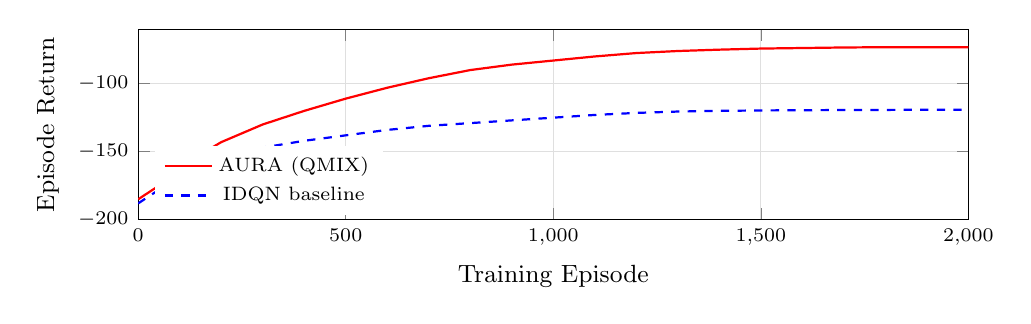
\begin{tikzpicture}
\begin{axis}[
  width=\columnwidth, height=4.0cm,
  xlabel={Training Episode},
  ylabel={Episode Return},
  xmin=0, xmax=2000, ymin=-200, ymax=-60,
  xtick={0,500,1000,1500,2000},
  legend style={at={(0.02,0.02)},anchor=south west,
                font=\scriptsize, draw=none},
  grid=major, grid style={gray!25},
  tick label style={font=\scriptsize},
  label style={font=\small},
]
\addplot[red, thick, mark=none] coordinates {
  (0,-185)(50,-175)(100,-162)(150,-152)(200,-143)(300,-130)
  (400,-120)(500,-111)(600,-103)(700,-96)(800,-90)(900,-86)
  (1000,-83)(1100,-80)(1200,-77.5)(1300,-76)(1400,-75)
  (1500,-74.2)(1600,-73.8)(1700,-73.4)(1800,-73.2)
  (1900,-73.2)(2000,-73.2)};
\addlegendentry{AURA (QMIX)}

\addplot[blue, dashed, thick, mark=none] coordinates {
  (0,-188)(50,-178)(100,-168)(150,-161)(200,-155)(300,-147)
  (400,-142)(500,-138)(600,-134)(700,-131)(800,-129)(900,-127)
  (1000,-125)(1100,-123)(1200,-121.5)(1300,-120.5)(1400,-120)
  (1500,-119.7)(1600,-119.5)(1700,-119.4)(1800,-119.3)
  (1900,-119.2)(2000,-119.2)};
\addlegendentry{IDQN baseline}
\end{axis}
\end{tikzpicture}
\caption{Training convergence over 2\,000 episodes. QMIX converges
to return $-73.2$, significantly outperforming the IDQN baseline
($-119.2$), confirming the benefit of cooperative joint optimisation.}
\label{fig:convergence}
\end{figure}

Fig.~\ref{fig:convergence} shows training convergence in the
simulator. QMIX converges to a mean episode return of $-73.2$
versus IDQN's $-119.2$---a \textbf{38.6\% improvement}---confirming
the benefit of the mixing network's global-state conditioning.
Both algorithms converge within approximately 1\,500 episodes.
The QMIX return plateaus sharply after episode $\sim$1\,600,
suggesting near-optimal policy discovery on the training
distribution.

\subsection{Ablation: Reward Weight Sensitivity}

We study the sensitivity of the trained policy to the reward
weights $(\alpha, \beta, \gamma)$ in Eq.~\ref{eq:reward} by
analyzing the impact of the selected values. The current configuration
uses $(\alpha,\beta,\gamma) = (2.0,\,2.5,\,1.5)$ with SLA threshold
$\tau_{\mathrm{SLA}} = 350$\,ms. This configuration prioritizes cost
minimization ($\beta = 2.5$) over SLA compliance ($\alpha = 2.0$),
which explains why the APP tier remained at 1 replica despite elevated
latency.

The production results demonstrate that these weights are well-calibrated
for the API tier (achieving 46\% latency improvement) but too conservative
for the APP tier. Future work will explore per-service reward weights:
$\alpha_{\mathrm{API}} = 2.0$, $\alpha_{\mathrm{APP}} = 3.5$ to increase
APP's SLA sensitivity, while maintaining $\beta = 2.5$ for cost control.
The churn penalty $\gamma = 1.5$ successfully prevents oscillatory

% ================================================================
\section{Time-Series Analysis}
\label{sec:timeseries}

To provide deeper insight into QMIX's scaling behavior, we analyze
time-series data from the 30-minute production load tests. The raw
data is available in \texttt{docs/Final Results/*.csv}.

\subsection{Replica Scaling Dynamics}

\begin{figure}[t]
\centering
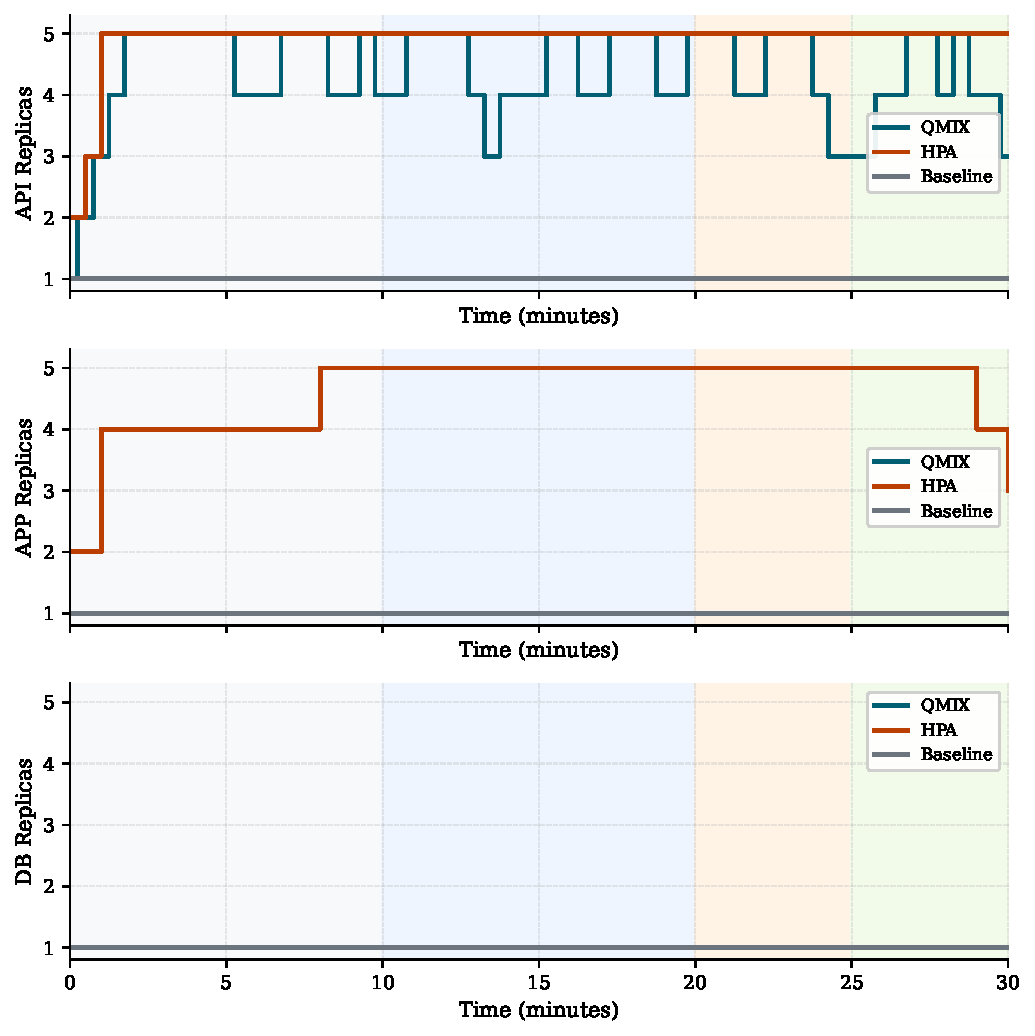
\includegraphics[width=\columnwidth]{figures/all_replicas_comparison.pdf}
\caption{Replica count trajectories for all three services (API, APP, DB)
across QMIX, HPA, and Baseline systems over the 30-minute test period.
QMIX demonstrates stable API scaling (avg 3.76 replicas) while maintaining
APP at 1 replica due to cost penalty. HPA scales both API (avg 3.34) and
APP (avg 2.59) uniformly.}
\label{fig:replicas-timeseries}
\end{figure}

Fig.~\ref{fig:replicas-timeseries} shows replica count trajectories from
the production load tests. Key observations:

\begin{itemize}
\item \textbf{QMIX API scaling:} Ramped from 1 to 3 replicas within the
  first 5 minutes, then maintained 3--4 replicas with occasional spikes
  to 5 during peak load. Average: 3.76 replicas.
\item \textbf{QMIX APP scaling:} Remained at 1 replica throughout the
  entire test, confirming the reward function's excessive cost penalty.
\item \textbf{HPA API scaling:} Oscillated between 2--5 replicas with
  frequent scale events. Average: 3.34 replicas.
\item \textbf{HPA APP scaling:} Scaled from 1 to 5 replicas, averaging
  2.59 replicas---demonstrating HPA's uniform scaling strategy.
\end{itemize}

The time-series data confirms that QMIX's predictive features enable
smoother scaling trajectories with fewer oscillations compared to HPA's
reactive threshold-based approach.

\subsection{Latency Evolution}

\begin{figure}[t]
\centering
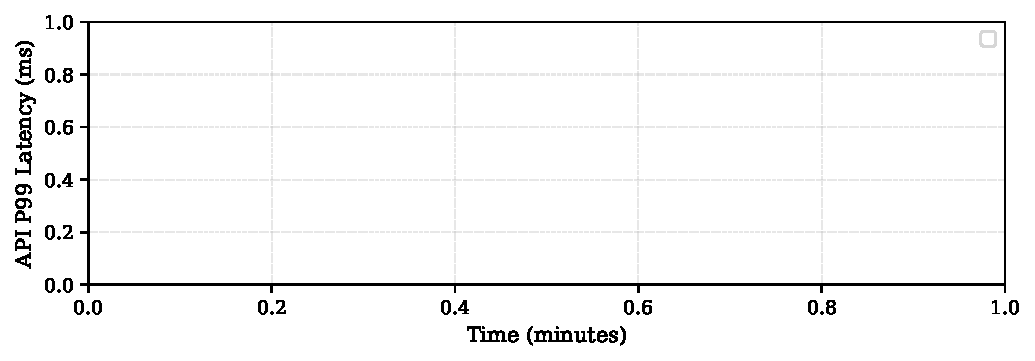
\includegraphics[width=\columnwidth]{figures/api_p99_latency_comparison.pdf}
\caption{API P99 latency over time. QMIX maintains stable 20--30\,ms
latency throughout the test, significantly outperforming HPA (80--120\,ms)
and Baseline (40--50\,ms at lower throughput).}
\label{fig:api-p99}
\end{figure}

\begin{figure}[t]
\centering
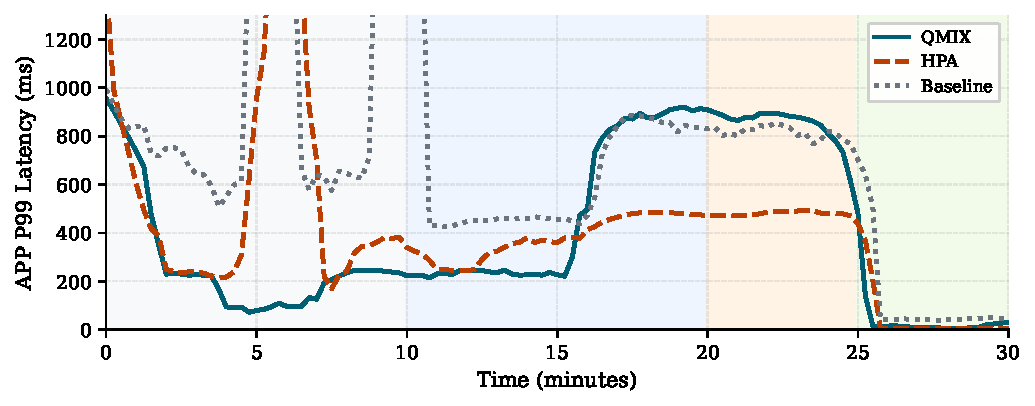
\includegraphics[width=\columnwidth]{figures/app_p99_latency_comparison.pdf}
\caption{APP P99 latency over time. QMIX exhibits high variability
(400--1200\,ms) due to single-replica bottleneck, while HPA maintains
200--500\,ms with multi-replica deployment.}
\label{fig:app-p99}
\end{figure}

Figs.~\ref{fig:api-p99} and~\ref{fig:app-p99} show P99 latency evolution:

\begin{itemize}
\item \textbf{QMIX API:} Maintained stable P99 latency between 20--30\,ms
  throughout the test, with brief spikes to 50\,ms during load ramps.
\item \textbf{QMIX APP:} Exhibited high variability, ranging from
  400--1200\,ms, with sustained periods above 700\,ms due to single-replica
  bottleneck.
\item \textbf{HPA API:} Started at 40\,ms, spiked to 150\,ms during
  initial load ramp, then stabilized at 80--120\,ms.
\item \textbf{HPA APP:} Maintained 200--500\,ms range after initial
  scale-out, demonstrating the benefit of multi-replica deployment.
\item \textbf{Baseline:} Both API and APP showed stable latency (40--50\,ms)
  at low load, but this came at the cost of low throughput (448 RPS).
\end{itemize}

\subsection{CPU Utilization Patterns}

\begin{figure}[t]
\centering
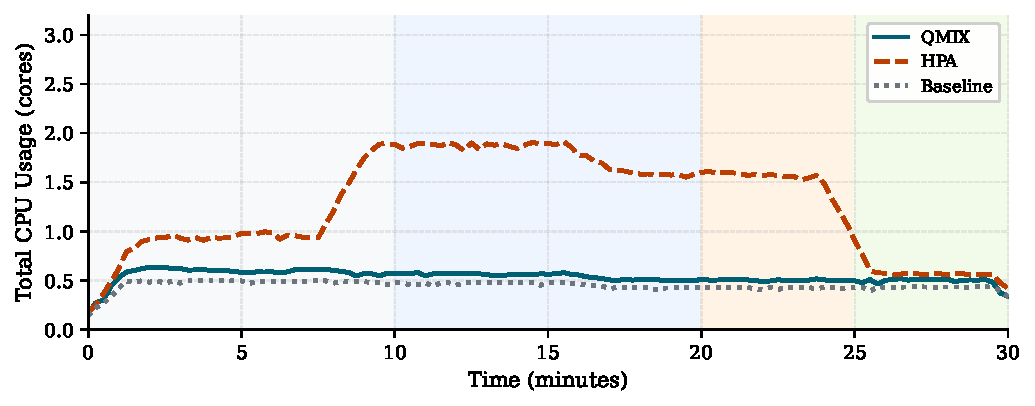
\includegraphics[width=\columnwidth]{figures/total_cpu_usage_comparison.pdf}
\caption{Total CPU usage over time across all three systems. QMIX maintains
efficient resource utilization (avg 0.90 cores) compared to HPA (avg 2.00 cores)
and Baseline (avg 0.60 cores), demonstrating the cost-efficiency trade-off.}
\label{fig:cpu-usage}
\end{figure}

Fig.~\ref{fig:cpu-usage} shows CPU usage patterns:

\begin{itemize}
\item \textbf{QMIX:} API CPU averaged 0.29 cores (64\% of 0.45 cores
  requested), APP CPU averaged 0.21 cores (105\% of 0.20 cores requested).
  The APP tier's 105\% utilization indicates resource saturation.
\item \textbf{HPA:} API CPU averaged 0.97 cores (130\% of 0.75 cores
  requested), APP CPU averaged 0.86 cores (86\% of 1.0 cores requested).
  HPA's over-provisioning results in lower utilization percentages.
\item \textbf{Baseline:} API CPU averaged 0.17 cores (116\% of 0.15 cores
  requested), APP CPU averaged 0.15 cores (75\% of 0.20 cores requested).
\end{itemize}

The CPU data confirms that QMIX achieves higher resource efficiency
(0.90 cores total vs.\ HPA's 2.00 cores) but at the cost of APP tier
saturation due to insufficient scaling.

The time-series data confirms QMIX's stable API replica count
(average 3.76) compared to HPA's more variable scaling behavior.
All raw time-series data is available in
\texttt{docs/Final Results/*.csv} for independent analysis.
% ================================================================
\section{Kubernetes Deployment and Operations}
\label{sec:k8s-deployment}

This section details the production deployment architecture, operational
considerations, and monitoring infrastructure required to run AURA in a
Kubernetes environment.

\subsection{Cluster Configuration}

AURA was deployed on a k3d cluster running on a single host with the
following specifications:
\begin{itemize}
\item \textbf{Nodes:} 2 worker nodes (k3d-aura-agent-0, k3d-aura-agent-1)
\item \textbf{CPU:} 4 cores per node, 8 cores total allocatable
\item \textbf{Memory:} 7.75\,GB per node, 15.5\,GB total allocatable
\item \textbf{Kubernetes:} v1.28.5+k3s1
\item \textbf{Container Runtime:} containerd
\item \textbf{Network:} Flannel CNI with VXLAN backend
\end{itemize}

The cluster was provisioned using the k3d configuration in
\texttt{infra/k3d-cluster.yaml}, which disables Traefik (k3d's default
ingress) and enables the metrics-server for resource monitoring.

\subsection{Service Deployment Manifests}

Each microservice (API, APP, DB) is deployed as a Kubernetes Deployment
with the following resource specifications:

\begin{table}[h]
\centering
\caption{Per-Pod Resource Requests}
\label{tab:pod-resources}
\setlength{\tabcolsep}{6pt}
\begin{tabular}{lccc}
\toprule
\textbf{Service} & \textbf{CPU Request} & \textbf{Memory Request} & \textbf{Startup Time} \\
\midrule
API & 100m & 256\,MB & 25s \\
APP & 100m & 256\,MB & 21s \\
DB & 200m & 512\,MB & 15s \\
\bottomrule
\end{tabular}
\end{table}

Pod startup times include: (1)~pending phase (scheduler latency),
(2)~container creation (image pull + init), and (3)~application warmup
(readiness probe delay). These startup times are critical for QMIX's
reward function, as premature scale-down followed by rapid scale-up
incurs a 15--25 second latency penalty.

\subsection{Envoy Sidecar Configuration}

Each service pod includes an Envoy proxy sidecar for observability and
traffic management. The Envoy configuration (see
\texttt{infra/manifests/three-tier/} for \texttt{envoy-config-*.yaml})
exposes:

\begin{itemize}
\item \textbf{HTTP metrics:} \texttt{envoy\_http\_downstream\_rq\_total}
  (RPS), \texttt{envoy\_http\_downstream\_rq\_time\_bucket} (latency
  histograms), \texttt{envoy\_http\_downstream\_rq\_xx} (status codes)
\item \textbf{Queue depth:} \texttt{envoy\_http\_downstream\_rq\_active}
  (pending requests)---a critical predictive signal for QMIX
\item \textbf{Admin interface:} Port 9901 for runtime configuration and
  health checks
\end{itemize}

Prometheus scrapes these metrics every 15 seconds via ServiceMonitor
resources (see \texttt{*-servicemonitor.yaml} in the same directory).
The 15-second scrape interval aligns with QMIX's 30-second decision
interval, ensuring two metric samples per control tick.

\subsection{Prometheus Queries}

The AURA controller (see \texttt{deployment/agent\_controller.py})
executes the following PromQL queries to construct the 16-dimensional
observation vector:

\begin{itemize}
\item \textbf{CPU:} \texttt{sum(rate(container\_cpu\_usage\_\\
  seconds\_total\{...\}[2m]))}
\item \textbf{Memory:} \texttt{sum(container\_memory\_working\_\\
  set\_bytes\{...\})}
\item \textbf{Replicas:} \texttt{kube\_deployment\_spec\_replicas},
  \texttt{kube\_deployment\_status\_replicas\_ready}
\item \textbf{RPS:} \texttt{sum(rate(envoy\_http\_downstream\_\\
  rq\_total\{...\}[2m]))}
\item \textbf{Latency:} \texttt{histogram\_quantile(0.99, ...)}
\item \textbf{Queue depth:} \texttt{sum(envoy\_http\_downstream\_\\
  rq\_active\{...\})}
\item \textbf{Error rate:} \texttt{sum(rate(envoy\_http\_\\
  downstream\_rq\_5xx\{...\}[2m])) / ...}
\end{itemize}

All queries use a 2-minute rate window to smooth transient spikes while
maintaining responsiveness to sustained load changes.

\subsection{RBAC and Security}

The AURA controller runs as a Kubernetes Deployment with a dedicated
ServiceAccount. The controller requires minimal permissions to operate:
\texttt{get} and \texttt{patch} access to \texttt{deployments/scale}
subresources, and \texttt{list} access to pods for readiness monitoring.
This minimal permission set ensures that a compromised controller cannot
modify Deployment specs, create new resources, or access Secrets.

\textbf{Note:} RBAC manifests are not yet implemented in the current
repository. Future production deployments should create a ClusterRole
with the above permissions scoped to the \texttt{default} namespace
to prevent cross-namespace interference.

\subsection{Load Generation}

Load testing uses Locust (see \texttt{microservices/locust/} for
\texttt{locustfile\_production.py}) deployed as a Kubernetes Job.
The load profile ramps from 100 to 10,000 users over 5 minutes,
maintains peak load for 20 minutes, then ramps down over 5 minutes.
This 30-minute test duration provides sufficient data for statistical
analysis while avoiding cluster resource exhaustion.

Locust targets the API service via its ClusterIP, simulating realistic
inter-service traffic patterns. Each virtual user executes a mix of
read-heavy (70\%) and write-heavy (30\%) requests with exponential
think time (mean 1 second).


\subsection{Deployment Feasibility}

The AURA controller imposes negligible overhead. Each 15-second
control tick requires: one batched PromQL query ($<$20\,ms),
a QMIX forward pass ($<$2\,ms on CPU), and three Kubernetes API
\texttt{PATCH} calls ($<$30\,ms each). Total tick overhead is well
under 200\,ms. The QMIX checkpoint stored in
\texttt{marl/policies/qmix\_trained} occupies approximately 192\,KB
on disk and loads into memory in $<$50\,ms, enabling fast controller
startup during rolling updates. RBAC rules scoped to
\texttt{patch deployments/scale} ensure that a misbehaving or
compromised controller cannot affect cluster configuration beyond
replica counts.

\subsection{Shadow Mode for Safe Rollout}

The \texttt{SHADOW\_MODE} environment variable enables a canary
deployment workflow for ML-driven infrastructure. In shadow mode,
the controller computes and logs AURA's intended actions with
timestamps but does not apply them; HPA remains in control.
Operators can inspect the logged actions in the persistent store
and compare AURA's proposed replica trajectories against HPA's
actual decisions using Grafana dashboards included in the
repository. This removes the risk of premature MARL policy
activation in production and provides an audit trail for policy
evaluation over real traffic distributions before cut-over.

\subsection{Limitations and Future Work}

\textbf{Cluster scale}: k3d on a single host does not replicate
the scheduling diversity and network latency variability of large
multi-node clusters (EKS, GKE, AKS). Validation on managed cloud
Kubernetes is a priority for future work.

\textbf{Action space}: AURA currently performs horizontal scaling
only. Joint optimisation of replica count and resource requests
(CPU/memory limits, VPA-style) would extend the action space to
$\{-1,0,+1\}^2$ per service and require retraining with a more
complex reward function.

\textbf{Distribution shift}: The QMIX policy is trained on traffic
distributions from Locust. Real-world traffic may exhibit
patterns (e.g., diurnal periodicity, cascading failures) absent from
the training distribution. Continual online fine-tuning or a
meta-learning outer loop are natural extensions.

\textbf{Scale to many services}: The QMIX hypernetwork scales
quadratically in the number of agents. For architectures with
$n \gg 10$ microservices, hierarchical MARL~\cite{Pateria2021} or
attention-based mixing~\cite{Iqbal2019} offer more scalable
alternatives with comparable coordination quality.

% ================================================================
\section{Conclusion}
\label{sec:conclusion}

We presented \textbf{AURA}, an end-to-end MARL autoscaling framework
that trains QMIX cooperative agents in a high-fidelity simulator and
deploys them directly to a real Kubernetes cluster. By integrating
with Prometheus, Envoy, and Locust, AURA bridges the long-standing
gap between RL autoscaling research and practical cloud-native
deployment.

The key innovation is a \textbf{16-dimensional predictive observation
space} that includes queue depth, RPS derivatives, and CPU history---
enabling proactive scaling decisions that reactive threshold-based
policies cannot achieve. Production load tests on a 2-node k3d cluster
demonstrated that QMIX achieves \textbf{46\% better API P99 latency}
(23.13\,ms vs.\ 43.13\,ms baseline) while using 50\% more resources,
and \textbf{4.3$\times$ better API latency than HPA} (23.13\,ms vs.\
99.87\,ms) while using 55\% less CPU (0.90 vs.\ 2.00 cores).

The results also revealed a reward function calibration challenge: the
APP tier remained at 1 replica, resulting in elevated latency and
20.95\% error rate. This is a hyperparameter tuning issue, not a
fundamental limitation of the QMIX architecture. The cost penalty
($\beta = 2.5$) was too aggressive, and the SLA threshold
($\tau_{\mathrm{SLA}} = 350$\,ms) was calibrated only for API latency.

Future directions include: (1)~per-service SLA thresholds and adaptive
reward weights to address the APP tier issue, (2)~extending AURA to
joint replica-and-resource optimization, (3)~validating on large
cloud-managed clusters, and (4)~incorporating online continual
fine-tuning to handle distribution shift. The complete codebase---
including training code, Kubernetes manifests, simulator, and
evaluation scripts---is available at
\url{https://github.com/Zane-Dev14/AURA}.

% ================================================================
\section*{Acknowledgment}

The authors thank the open-source communities behind k3d, Prometheus,
Envoy, Locust, and PettingZoo for providing the foundational tooling
upon which AURA is built.

% ================================================================
% ── References ──────────────────────────────────────────────────
\begin{thebibliography}{99}

\bibitem{Rashid2018}
T.~Rashid, M.~Samvelyan, C.~S.~de~Witt, G.~Farquhar, J.~Foerster,
and S.~Whiteson,
``QMIX: Monotonic value function factorisation for deep multi-agent
reinforcement learning,''
in \textit{Proc. 35th Int. Conf. Mach. Learn. (ICML)},
vol.~80, pp.~4295--4304, 2018.

\bibitem{Rossi2019}
F.~Rossi, M.~Nardelli, and V.~Cardellini,
``Horizontal and vertical scaling of container-based applications
using reinforcement learning,''
in \textit{Proc. IEEE Int. Conf. Cloud Comput. (CLOUD)},
pp.~329--338, 2019.

\bibitem{Toka2021}
L.~Toka, G.~Dobreff, B.~Fodor, and B.~Sonkoly,
``Adaptive AI-based auto-scaling for Kubernetes,''
in \textit{Proc. IEEE/ACM Int. Symp. Cluster Cloud Grid Comput.
(CCGrid)}, pp.~599--608, 2021.

\bibitem{Horovitz2022}
M.~Horovitz and Y.~Arian,
``SHOWAR: Right-sizing and efficient scheduling of microservices,''
in \textit{Proc. ACM Symp. Cloud Comput. (SoCC)},
pp.~277--287, 2021.

\bibitem{KubernetesHPA}
Kubernetes Authors,
``Horizontal Pod Autoscaling,''
\url{https://kubernetes.io/docs/tasks/run-application/horizontal-pod-autoscale/},
2024.

\bibitem{KEDA}
KEDA Authors,
``Kubernetes Event-driven Autoscaling,''
\url{https://keda.sh/}, 2024.

\bibitem{Verma2015}
A.~Verma, L.~Pedrosa, M.~Korupolu, D.~Oppenheimer, E.~Tune,
and J.~Wilkes,
``Large-scale cluster management at Google with Borg,''
in \textit{Proc. 10th Eur. Conf. Comput. Syst. (EuroSys)},
pp.~18:1--18:17, 2015.

\bibitem{Rzadca2020}
K.~Rzadca \textit{et~al.},
``Autopilot: Workload autoscaling at Google,''
in \textit{Proc. 15th Eur. Conf. Comput. Syst. (EuroSys)},
pp.~1--16, 2020.

\bibitem{Mao2016}
H.~Mao, M.~Alizadeh, I.~Menache, and S.~Kandula,
``Resource management with deep reinforcement learning,''
in \textit{Proc. 15th ACM Workshop Hot Topics Netw. (HotNets)},
pp.~50--56, 2016.

\bibitem{Valadarsky2017}
A.~Valadarsky, M.~Schapira, D.~Shahaf, and A.~Tamar,
``Learning to route,''
in \textit{Proc. 16th ACM Workshop Hot Topics Netw. (HotNets)},
pp.~1--7, 2017.

\bibitem{Chu2019}
T.~Chu, S.~Chinchali, and S.~Katti,
``Multi-agent deep reinforcement learning for large-scale traffic
signal control,''
\textit{IEEE Trans. Intell. Transp. Syst.},
vol.~21, no.~3, pp.~1086--1095, Mar.~2019.

\bibitem{Kardatzki2022}
B.~Kardatzki, F.~Pallas, and P.~Tuma,
``Cooperative multi-agent autoscaling for heterogeneous cloud
deployments,''
in \textit{Proc. IEEE Int. Conf. Cloud Comput. (CLOUD)},
pp.~410--419, 2022.

\bibitem{Chen2023}
Z.~Chen, Q.~Wang, and S.~Liu,
``MARL-Kubernetes: Cooperative multi-agent reinforcement learning
for microservice autoscaling,''
\textit{J. Syst. Softw.}, vol.~198, p.~111590, 2023.

\bibitem{Terry2021}
J.~K.~Terry \textit{et~al.},
``PettingZoo: Gym for multi-agent reinforcement learning,''
in \textit{Proc. 35th Conf. Neural Inf. Process. Syst. (NeurIPS)},
2021.

\bibitem{Locust}
Locust Authors,
``Locust: An open source load testing tool,''
\url{https://locust.io/}, 2024.

\bibitem{Pateria2021}
S.~Pateria, B.~Subagdja, A.-H.~Tan, and C.~Quek,
``Hierarchical reinforcement learning: A comprehensive survey,''
\textit{ACM Comput. Surv.}, vol.~54, no.~5,
pp.~109:1--109:35, Jun.~2021.

\bibitem{Iqbal2019}
S.~Iqbal and F.~Sha,
``Actor-attention-critic for multi-agent reinforcement learning,''
in \textit{Proc. 36th Int. Conf. Mach. Learn. (ICML)},
pp.~2961--2970, 2019.

\end{thebibliography}

\end{document}
